% !TeX spellcheck = en_US
\documentclass[
english,
openany,
draft = false,
twoside = true,
fleqn
]{scrbook}
\usepackage{learning-notes}

\author{Huu Duc Nguyen}
\authordegreefront{}
\authordegreeback{ M.Sc.}
\subject{Computer Vision}
\title{Computer Vision Notes}
\date{29 March 2022}

\begin{document}
	\frontmatter
	\TitlePage
	\tableofcontents
	
	\mainmatter
	% !TeX spellcheck = en_GB

\chapter*{Abbreviations}
\addcontentsline{toc}{chapter}{Abbreviations}

\begin{acronym}[LONGEST]
	\acro{AI}{Artificial Intelligence}
	\acro{ML}{Machine Learning}
	\acro{DL}{Deep Learning}
	\acro{CS}{Computer Science}
	\acro{CV}{Computer Vision}
	\acro{RL}{Reinforcement Learning}
	\acro{NLP}{Natural Language Processing}
	
	\acro{prob}[prob.]{probability}
	\acro{param}[params.]{parameters}
	\acro{algor}[algor.]{algorithms}
	\acro{info}[info.]{information}
	\acro{aka}[a.k.a.]{also known as}
	\acro{no}[no.]{number of}
	\acro{func}[func.]{function}
	\acro{vs}[vs.]{versus}
	\acro{iid}[i.i.d.]{independent \& identically distributed}
	\acro{LSI}{linear shift invariant}
	
	\acro{pdf}[PDF]{Probability Density Function}
	\acro{MLE}{Maximum Likelihood Estimation}
	\acro{MAP}{Maximum A Posteriori}

	\acro{MoG}{Mixture of Gaussians}
	
	% Gradient descent
	\acro{nag}[NAG]{Nestorov Accelerated Gradient}
	\acro{rmsprop}[RMSprop]{Root mean squared prop}
	\acro{adam}[Adam]{Adaptive moment estimation}
	
	\acro{SVD}{Singular Value Decomposition}
	\acro{PCA}{Principal Component Analysis}
	\acro{LDA}{Linear Discriminant Analysis}
	\acro{kl}[K-L]{Kullback–Leibler}
	
	% Neural-network-related term
	\acro{relu}[ReLU]{Rectified Linear Unit}
\end{acronym}
	% !TeX spellcheck = en_US
\chapter{Introduction}
\label{cha:intro}

\hlb{Goal:} The goal of computer vision is enabling machine to understand images \& videos. There are two major tasks:
\begin{itemize}
	\item measurement: compute properties of 3D world (distance, shape)
	\item perception \& interpretation: recognize objects, people, activities, ..
\end{itemize}

\hlb{Outlines}
\begin{itemize}
	\item \charef{cha:math-cv} presents mathematics backgrounds for computer vision
	\item \todo{\charef{} do sth}
\end{itemize}
	% !TeX spellcheck = en_US
\chapter{Mathematics Backgrounds}
\label{cha:math-cv}
This chapter presents some mathematics backgrounds.

\section{The Matrix Equation}
\hlb{Problem:} Solve $Ax=0$
\begin{itemize}
	\item Applying \ac{SVD} for matrix $A$
	\[ A = U.D.V^T = U. \begin{bmatrix}
		d_{11} & \cdots & d_{1N}\\
		\vdots & \ddots & \vdots\\
		d_{N1} & \cdots & d_{NN}
	\end{bmatrix} . \begin{bmatrix}
		v_{11} & \cdots & v_{1N}\\
		\vdots & \ddots & \vdots\\
		v_{N1} & \cdots & v_{NN}
	\end{bmatrix}^T	\]
	\item Solution of $Ax=0$ is the null space vector of $A$, which corresponds to the smallest (last) singular vector of $A$: $ \left[ v_{1N}, \cdots, v_{NN} \right]^T$.
\end{itemize}
	
	% !TeX spellcheck = en_US
\chapter{Image Formation}
\label{cha:image-formation}

\section{Camera Obscura}
\ac{aka} the "Dark Chamber" (Leonardo Da Vinci, 1545)
\begin{figure}[hbt!]
	\centering
	\includegraphics[width=0.79\textwidth]{camera-obscura.jpg}
	\caption{Camera obscura \cite{frisiusradio}.}
\end{figure}

\section{Pinhole Camera}
\begin{itemize}
	\item Pinhole size $=$ aperture
	\begin{itemize}
		\item too big $\Rightarrow$ blurring
		\item too small $\Rightarrow$ also blur, but because of diffraction\\ but then, \hlb{image is dark}
	\end{itemize}
	$\Rightarrow$ Use lenses: keep image sharp while \hlb{capture more light}
	\item The thin lens
	\item Focus \& Depth of Field:
	\begin{itemize}
		\item Large aperture: small depth of field\\
		(only object within the correct distance will be at focus, while background is blur)
		\item Small aperture: large depth of field, but need more light
	\end{itemize}
	\item The lens focus $f \gtrless$ field of view
	\begin{figure}[hbt!]
		\centering
		\includegraphics[width=0.57\textwidth]{depth-of-field.png}
		\caption{Varied depths of field depending on aperture size.}
	\end{figure}
	\begin{itemize}
		\item $f$ gets smaller $\Rightarrow$ wide-range image
		\item $f$ gets greater $\Rightarrow$ telescopic image
	\end{itemize}
\end{itemize}

\section{Digital image}
\begin{itemize}
	\item Discretize the image into a grid of pixels
	\item Quantize light intensities $\Rightarrow$ pixel values
	\item Resolution: \ac{no} pixels (most commonly understand)
\end{itemize}

\section{Color Sensing}
Referring to the process of assigning pixel values from color information of world objects.
\begin{itemize}
	\item Color image: RGB is just 1 of many color spaces, \eg, LUV, XYZ (\href{https://en.wikipedia.org/wiki/List_of_color_spaces_and_their_uses}{Wikipedia}).
	\item Grey-scale image
\end{itemize}

\subsection{Demosaicing}
Digital camera takes in light through a filter (Bayer or Xtrans) $\Rightarrow$ we get a gray-scale image (\figref{fig:demosaicing}). We need to apply demosaicing based on the filter's pattern to get the color image from the raw image. Sources: \href{https://www.youtube.com/watch?v=9cPxEFpg3Eg}{YouTube}, \href{https://en.wikipedia.org/wiki/Demosaicing}{Wikipedia}.
\begin{figure}[hbt!]
	\centering
	\includegraphics[width=\textwidth]{demosaicing.png}
	\caption{\Eg Bayer Filter. In the raw image , which lies below the filter layers, each pixel only has \ac{info} of only 1 among 3 light sources. Demosaicing uses the values of surrounding pixels to infer the brightness of other light sources.}
	\label{fig:demosaicing}
\end{figure}

\note Raw image has a \hlb{green cast}\\
Twice many green as red \& blue, because human eyes are twice as sensitive to the green part to other red or blue part.

	% !TeX spellcheck = en_US
\chapter{Image Processing}

\section{Linear Filters}
Types of noise:
\begin{itemize}
	\item Salt \& pepper noise
	\item Impulse noise
	\item Gaussian noise\\
	$noise = randn(size(img)) \times \sigma$\\
	$output = img + noise$
	\item \hlr{\underline{Basic assumption:}} \ac{iid}
\end{itemize}
Types of filter:
\begin{itemize}
	\item Correlation Filter: $\displaystyle G[i,j] = \frac{1}{(2k+1)^2} \sum_{u=-k}^{k} \sum_{v=-k}^{k} F[i+u, j+v] $\\
	different weights: $\displaystyle G[i,j] = \sum_{u=-k}^{k} \sum_{v=-k}^{k} H[u,v]F[i+u, j+v] \Rightarrow {\color{red} \boxed{G = H \otimes F}}$\\
	with $H[u,v]$ as non-uniform weights\\
	\hlb{Matlab:} \texttt{filter2, imfilter}
	\item Convolution: \tab $\displaystyle G[i,j] = \sum_{u=-k}^{k} \sum_{v=-k}^{k} H[u,v]F[i-u, j-v] \Rightarrow {\color{red} \boxed{G = H * F}}$\\
	\hlb{Matlab:} \texttt{conv2}\\
	\hlr{If $H[u,v] = H[-u,-v] \Rightarrow$ correlation $\equiv$ convolution}
	\item Averaging Filter: \hlr{Ringing Artifacts??}
	\item Gaussian Filter: $\displaystyle \frac{1}{\sqrt{2\pi}} \exp \left(-\frac{(x-\mu)^2}{2\sigma^2}\right)$\\
	\hlb{Rule of thumb:} set the filter width to $6\sigma$\\
	\hlr{More noise $\Rightarrow\;\; \uparrow \sigma \Rightarrow$ blurring effect}
\end{itemize}

\note
\begin{itemize}
	\item \hlr{$k$ is from the window size $(2k+1)\times(2k+1)$}
	\item \hlr{Efficient implementation:} if filter is separable $\Rightarrow$ apply 1D filter 2 times to have a 2D filter $\Rightarrow$ Reduce the computational cost from $\mathcal{O}(K^2)$ to $\mathcal{O}(2K)$, with $K$ as the kernel size
	\item When coding with \texttt{Python}, the origin of image plane is top left corner, $x$-axis goes left, $y$-axis goes downward (\figref{fig:image-coords})
	\begin{figure}[!htb]
		\centering
		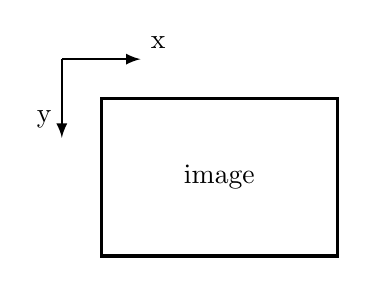
\begin{tikzpicture}			
			\draw[thick,-latex] (0,0) -- (1,0) node[anchor=south west] {x};
			\draw[thick,-latex] (0,0) -- (0,-1) node[anchor=south east] {y};
			\draw[very thick] (0.5,-0.5)  rectangle (3.5,-2.5) node[pos=.5]{image};
		\end{tikzpicture}
		\caption{Image coordinate system in \texttt{Python}}	
		\label{fig:image-coords}
	\end{figure}
	\item Boundary issues:
	\begin{align*}
		&\text{- Full: }  \tab \text{output size} = f+g && 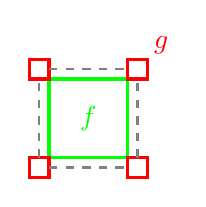
\begin{tikzpicture}[scale=0.5]\draw[green, very thick] (0,0) rectangle (2,2) node[pos=.5]{$f$};
			\draw[red, very thick] (2,2) rectangle (2.5,2.5) node[pos=1.7]{$g$};
			\draw[red, very thick] (0,0) rectangle (-.5,-.5);
			\draw[red, very thick] (2,0) rectangle (2.5,-.5);
			\draw[red, very thick] (0,2) rectangle (-.5,2.5);
			\draw[gray, thick, dashed] (-.25,0) -- (-.25,2);
			\draw[gray, thick, dashed] (0,-.25) -- (2,-.25);
			\draw[gray, thick, dashed] (2.25,0) -- (2.25,2);
			\draw[gray, thick, dashed] (0,2.25) -- (2,2.25);
		\end{tikzpicture}\\
		&\text{- Same:}  \tab \text{output size} = f   && 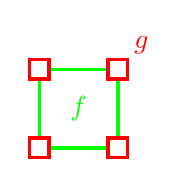
\begin{tikzpicture}[scale=0.5]\draw[green, very thick] (0,0) rectangle (2,2) node[pos=.5]{$f$};
			\draw[red, very thick, fill=white] (1.75,1.75) rectangle (2.25,2.25) node[pos=1.7]{$g$};
			\draw[red, very thick, fill=white] (1.75,-.25) rectangle (2.25,.25);
			\draw[red, very thick, fill=white] (-.25,-.25) rectangle (.25,.25);
			\draw[red, very thick, fill=white] (-.25,1.75) rectangle (.25,2.25);
		\end{tikzpicture}\\
		&\text{- Valid:} \tab \text{output size} = f-g && 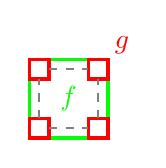
\begin{tikzpicture}[scale=0.5]\draw[green, very thick] (0,0) rectangle (2,2) node[pos=.5]{$f$};
			\draw[red, very thick] (1.5,1.5) rectangle (2,2) node[pos=1.7]{$g$};
			\draw[red, very thick] (0,0) rectangle (.5,.5);
			\draw[red, very thick] (2,0) rectangle (1.5,.5);
			\draw[red, very thick] (0,2) rectangle (.5,1.5);
			\draw[gray, thick, dashed] (.5,.25) -- (1.5,0.25);
			\draw[gray, thick, dashed] (.25,.5) -- (.25,1.5);
			\draw[gray, thick, dashed] (1.75,.5) -- (1.75,1.5);
			\draw[gray, thick, dashed] (.5,1.75) -- (1.5,1.75);
		\end{tikzpicture}
	\end{align*}
	\hlb{Pixel near boundary}:
	\begin{itemize}
		\item Clip filter (black) $\Rightarrow$ dark border
		\item Wrap around
		\item Copy edge $\Rightarrow$ Strong edge response
		\item Reflect across edge
	\end{itemize}
	\item Correlation \ac{vs} convolution:
	\begin{itemize}
		\item Both are linear shift invariant \ac{LSI}:\\
		\tab $h \circ (f_0 + f_1) = h \circ f_1 + h \circ f_0$
		\item Conv is better, it has additional nice properties
		\begin{itemize}
			\item commutative: $f*g = g*f$
			\item associative: $(f*g)*h = f*(g*h)$
			\item Fourier transform $f*g \multimap F.G$ and $f.h \multimap F*H$
		\end{itemize}
		\item With impulse image, Conv reproduces itself, while Corr reflects itself.
	\end{itemize}	
\end{itemize}

\section{Background}
\label{sec:filter-background}
\begin{itemize}
	\item Taking the Fourier Transform of a signal $\Rightarrow$ Frequency coefficients $\Rightarrow$ \hlb{Frequency Spectrum}\\
	\hlr{\underline{Duality:}} $\;$The \hlr{better} a function is \hlr{localized} in one domain\\
	\tab\tab the \hlr{worse} it is \hlr{localized} in the other domain.
	\item Effect of Convolution: $ f * g \multimap F \cdot G$\\
	taking convolution in one domain is equivalent to multiplication in the other domain\\
	A Guassian has compact support in both domains\\
	$\Rightarrow$ \hlb{convenient choice} for \hlr{low-pass filter}
	\item Sharpening filter \hlr{(high-pass filter)}: emphasizes noise as well, since noise is high \ac{freq} signal.
\end{itemize}
\begin{figure}[!htb]
	\centering
	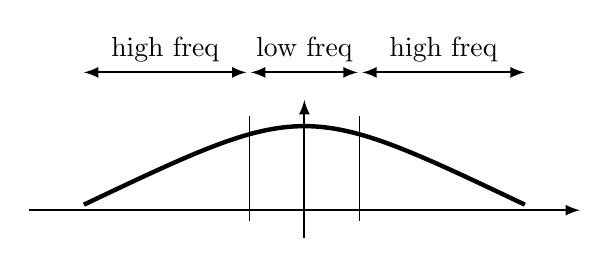
\begin{tikzpicture}[scale=0.7]
		\draw[thick,-latex] (-5,0) -- (5,0);
		\draw[thick,-latex] (0,-.5) -- (0,2);
		\draw[ultra thick] (-4,.1) .. controls (0,2) .. (4,.1);
		\draw[thin] (-1,-.2) -- (-1,1.7);
		\draw[thin] (1,-.2)  -- (1,1.7);
		\draw[thick,latex-latex] (-4,2.5) -- (-1.05,2.5) node[pos=0.5, above=0.2]{high \ac{freq}};
		\draw[thick,latex-latex] (1.05,2.5) -- (4,2.5) node[pos=0.5, above=0.2]{high \ac{freq}};
		\draw[thick,latex-latex] (-0.97,2.5) -- (0.97,2.5) node[pos=0.5, above=0.2]{low \ac{freq}};
	\end{tikzpicture}
	\caption{Frequency domain (Fourier).}
	\label{fig:freq-domain}
\end{figure}

\section{Non-Linear Filters}
\begin{itemize}
	\item Median filter: replace each pixel by the median of the neighbors.
	\begin{itemize}
		\item \hlr{remove spikes} (good for impulse, salt \& pepper noise)
		\item \hlr{edge preserving} (unlike mean filter)
	\end{itemize}
	\note If we increase the Median filter's filter size $\Rightarrow$ reduce structure and loose details
\end{itemize}

\section{Multi-Scale Representations}
\begin{itemize}
	\item Image pyramid: very \hlb{little overhead} (in terms of \hlb{computational cost}).
	\item \hlb{Fourier Interpretation:} Discrete Sampling\\
	Sampling in spatial domain is like \hlb{multiplying with a spike \ac{func}}.
	
	\begin{figure}[!htb]
		\centering
		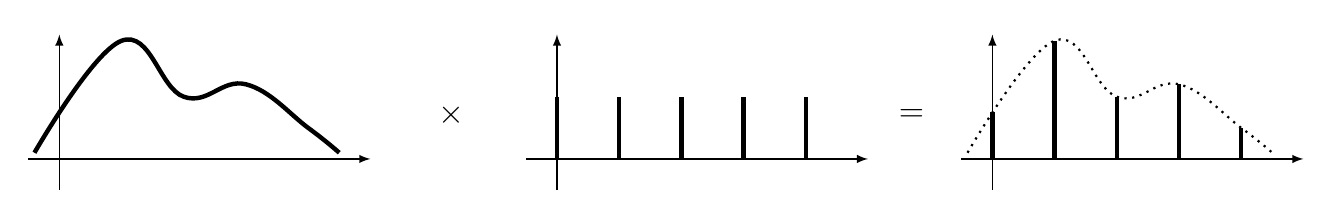
\begin{tikzpicture}[scale=0.79]
			\draw[-latex] (-.5,0) -- (5,0);
			\draw[-latex] (0,-.5) -- (0,2);
			\draw[ultra thick] plot [smooth, tension=.7] coordinates {(-.4,.1) (1,1.9) (2,1) (3,1.2) (4, .5) (4.5,0.1)};
			\node at (6.3,.7) {\large{$\boldsymbol{\times}$}};
			\draw[-latex] (7.5,0) -- (13,0);
			\draw[-latex] (8,-.5) -- (8,2);
			\draw[ultra thick] (8 ,0) -- (8 ,1);
			\draw[ultra thick] (9 ,0) -- (9 ,1);
			\draw[ultra thick] (10,0) -- (10,1);
			\draw[ultra thick] (11,0) -- (11,1);
			\draw[ultra thick] (12,0) -- (12,1);		
			\node at (13.7,.7) {\large{$\boldsymbol{=}$}};
			
			\draw[-latex] (14.5,0) -- (20,0);
			\draw[-latex] (15,-.5) -- (15,2);
			\draw[dotted, thick] plot [smooth, tension=.7, dashed] coordinates {(14.6,.1) (16,1.9) (17,1) (18,1.2) (19, .5) (19.5,.1)};
			\draw[ultra thick] (15,0) -- (15,.75);
			\draw[ultra thick] (16,0) -- (16,1.9);
			\draw[ultra thick] (17,0) -- (17,1);
			\draw[ultra thick] (18,0) -- (18,1.2);
			\draw[ultra thick] (19,0) -- (19,.5);
		\end{tikzpicture}
	\end{figure}
	
	$\Rightarrow$ Sampling in the frequency domain is like \hlb{convolving with a spike \ac{func}}.
	\begin{figure}[!htb]
		\centering
		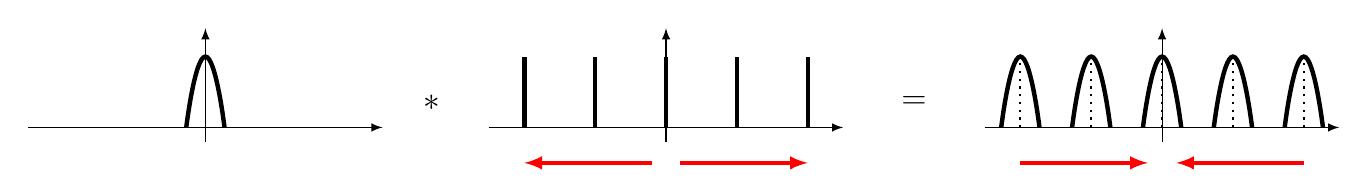
\begin{tikzpicture}[scale=0.9]
			\draw[-latex] (-2.5,0) -- (2.5,0);
			\draw[-latex] (0,-.2) -- (0,1.4);
			\draw[ultra thick] plot [smooth, tension=1] coordinates {(-.27,0) (0,1) (.27,0)};		
			\node at (3.2,.35) {\large{$\boldsymbol{\ast}$}};
			\draw[-latex] (4,0) -- (9,0);
			\draw[-latex] (6.5,-.2) -- (6.5,1.4);
			\draw[ultra thick] (4.5,0) -- (4.5,1);
			\draw[ultra thick] (5.5,0) -- (5.5,1);
			\draw[ultra thick] (6.5,0) -- (6.5,1);
			\draw[ultra thick] (7.5,0) -- (7.5,1);
			\draw[ultra thick] (8.5,0) -- (8.5,1);
			\node at (10 ,.35) {\large{$\boldsymbol{=}$}};		
			\draw[-latex] (11,0) -- (16,0);
			\draw[-latex] (13.5,-.2) -- (13.5,1.4);
			\draw[dotted, thick] (11.5,0) -- (11.5,1);
			\draw[dotted, thick] (12.5,0) -- (12.5,1);
			\draw[dotted, thick] (13.5,0) -- (13.5,1);
			\draw[dotted, thick] (14.5,0) -- (14.5,1);
			\draw[dotted, thick] (15.5,0) -- (15.5,1);
			\draw[ultra thick] plot [smooth, tension=1] coordinates {(11.23,0) (11.5,1) (11.77,0)};
			\draw[ultra thick] plot [smooth, tension=1] coordinates {(12.23,0) (12.5,1) (12.77,0)};
			\draw[ultra thick] plot [smooth, tension=1] coordinates {(13.23,0) (13.5,1) (13.77,0)};
			\draw[ultra thick] plot [smooth, tension=1] coordinates {(14.23,0) (14.5,1) (14.77,0)};
			\draw[ultra thick] plot [smooth, tension=1] coordinates {(15.23,0) (15.5,1) (15.77,0)};
			\draw[red, latex-, very thick] (4.5,-.5) -- (6.3,-.5);
			\draw[red, -latex, very thick] (6.7,-.5) -- (8.5,-.5);
			\draw[red, -latex, very thick] (11.5,-.5) -- (13.3,-.5);
			\draw[red, latex-, very thick] (13.7,-.5) -- (15.5,-.5);		
		\end{tikzpicture}
	\end{figure}\\
	$\Rightarrow$ when we sampling with lower \ac{freq}, the spikes will get further from each others. Due to duality in \secref{sec:filter-background}, the magnitude spectrum will be overlapped $\Rightarrow$ we will not be able to reconstruct the original signal / data.
	\item \hlb{Nyquist theorem and limit:} to recover a certain \ac{freq} $f$, you have to take sample with at least with $2f$.\\	
	\hlr{$\Rightarrow$ Aliasing artifacts in Graphics:} overlapped signal (because sampling with too low frequency)\\	
	\note We can't recover high \ac{freq} (edges), but we can \hlb{avoid artifacts} by \hlb{prior smoothing} before sampling.
	\item The Gaussian Pyramid:	perform blurring \& smoothing $\Rightarrow$ then down-sampling \todo{Image}
	\item The Laplacian Pyramid: \todo{Image}
	\begin{align*}
		L_i &= G_i - expand(G_{i+1})\\
		G_i &= L_i + expand(G_{i+1})\\
		L_n &= G_n
	\end{align*}
	$\Rightarrow L_{0} \rightarrow L_{n-1}$ contain \hlb{high \ac{freq} \ac{info}}\\
	\note Images in Laplacian Pyramid \hlb{can be compressed further} than the corresponding Gaussian Pyramid images.
	\item \hlr{Laplacian $\sim$ Difference of Gaussians}\\
	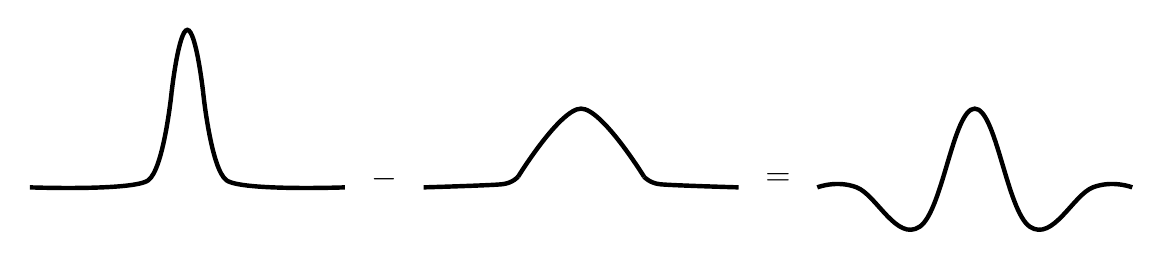
\begin{tikzpicture}
		\draw[ultra thick] plot [smooth, tension=1] coordinates {(-.2,1.21) (0,2) (.2,1.21)};
		\draw[ultra thick] plot [smooth, tension=.4] coordinates {(-2,0) (-.5,.0876) (-.2,1.21)};
		\draw[ultra thick] plot [smooth, tension=.4] coordinates {(.2,1.21) (.5,.0876) (2,0)};
		\node at (2.5,.1) {\large{$\boldsymbol{-}$}};
		\draw[ultra thick] plot [smooth, tension=.6] coordinates {(-.8+5,.135) (0+5,1) 	  (.8+5,.135)};		
		\draw[ultra thick] plot [smooth, tension=.4] coordinates {(-2 +5,0)   (-1+5,.04) (-.8+5,.135)};
		\draw[ultra thick] plot [smooth, tension=.4] coordinates {(.8 +5,.135) (1+5,.04)   (2+5,0)};
		\node at (7.5,.1) {\large{$\boldsymbol{=}$}};
		\draw[ultra thick] plot [smooth, tension=.7] coordinates {(-2+10,0) (-1.5+10,0) (-.7+10,-.5) (0+10,1) (.7+10,-.5) (1.5+10,0) (2+10,0)};
	\end{tikzpicture}\\
	$\Rightarrow$ detect high-\ac{freq} $\approx$ edges\\
	The name Laplace $\Rightarrow$ from a combinations of 2nd derivatives\\
	Laplacian: $\displaystyle {\color{red} \boxed{\nabla^2f = \frac{\partial^2f}{\partial x^2} + \frac{\partial^2f}{\partial y^2}}}$
	\begin{align*}
		\frac{\partial^2f}{\partial x^2} &= [f(x+1,y) - f(x,y)] - [f(x,y) - f(x-1,y)] \\
		&= f(x+1,y) + f(x-1,y) - 2f(x,y) \\
		\Rightarrow \nabla^2f &= f(x\pm1, y) + f(x, y\pm1) - 4f(x,y) \\
	\end{align*}
	$\Rightarrow$ \hlb{Laplacian filter:} \tab 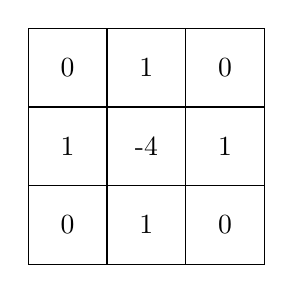
\begin{tikzpicture}
		\draw (0,0) rectangle (1,1) node[pos=.5]{0};
		\draw (1,1) rectangle (2,2) node[pos=.5]{-4};
		\draw (2,2) rectangle (3,3) node[pos=.5]{0};
		\draw (1,0) rectangle (2,1) node[pos=.5]{1};
		\draw (2,0) rectangle (3,1) node[pos=.5]{0};
		\draw (0,1) rectangle (1,2) node[pos=.5]{1};
		\draw (0,2) rectangle (1,3) node[pos=.5]{0};
		\draw (1,2) rectangle (2,3) node[pos=.5]{1};
		\draw (2,1) rectangle (3,2) node[pos=.5]{1};
	\end{tikzpicture}	 
\end{itemize}

\section{Filters as Templates}
Correlation filtering as Template Matching.

\section{Image Gradients}
\begin{itemize}
	\item Differentiation \& Convolution: $\displaystyle \frac{\partial f(x,y)}{\partial x} \approx \frac{f(x+1,y) - f(x,y)}{1}$\\
	$\Rightarrow$ Filter: $\begin{bmatrix}
		1 & -1
	\end{bmatrix}$\\
	\hlb{Problem:} it shifts the image \\
	$\Rightarrow$ Prewitt, Sobel, Robert filters:
	\begin{itemize}
		\item Prewitt filter: $\begin{bmatrix}
			-1 & 0 & 1\\
			-1 & 0 & 1\\
			-1 & 0 & 1
		\end{bmatrix}; \begin{bmatrix}
			1 & 1 & 1\\
			0 & 0 & 0\\
			-1 & -1 & -1
		\end{bmatrix}$
		\item Sobel filter: $M_x=\begin{bmatrix}
			-1 & 0 & 1\\
			-2 & 0 & 2\\
			-1 & 0 & 1
		\end{bmatrix}; M_y=\begin{bmatrix}
			1 & 2 & 1\\
			0 & 0 & 0\\
			-1 & -2 & -1
		\end{bmatrix}$
		\item Robert $\begin{bmatrix}
			0 & 1\\
			-1 & 0
		\end{bmatrix}; \begin{bmatrix}
		1 & 0\\
		0 & -1
	\end{bmatrix}$
	\end{itemize}
	\item With noise, we need to smooth the image first
\end{itemize}

\section{Edge Detection}


\section{Structure Extraction}

\todo{missing content}
	% !TeX spellcheck = en_US
\chapter{Segmentation}
\todo{}
	% !TeX spellcheck = en_US
\chapter{Object Detection}
\todo{}
	% !TeX spellcheck = en_US
\chapter{Local Feature}
\todo{}
	% !TeX spellcheck = en_US
\chapter{Deep Learning for CV}
\todo{}

\section{Image-to-Image Translation}
Image-to-image translation is a class of computer vision problems where the goal is to learn the mapping between an input image and an output image. Recent approaches utilize \ac{GAN}. It has various applications \cite{isola2017image, zhu2017unpaired}, \eg:
\begin{itemize}
	\item Domain adaptation
	\item Semantic label $\leftrightarrow$ photo
	\item Map $\leftrightarrow$ aerial photo
	\item Edges $\rightarrow$ photo
	\item BW $\rightarrow$ color photos
	\item Day $\rightarrow$ night
	\item Photo with missing pixels $\rightarrow$ inpainted photo (recovering)
\end{itemize}

\subsection{pix2pix}
\texttt{pix2pix} uses \ac{CGAN} idea with U-Net architecture \cite{isola2017image}.
\begin{figure}[hbt!]
	\centering
	\includegraphics[width=0.9\textwidth]{pix2pix.png}
	\caption{Training a \ac{CGAN} to map edges $\rightarrow$ photo. Both the discriminator and generator are conditioned on the input $x$. \cite{isola2017image}}
\end{figure}

The loss function of \texttt{pix2pix} combines \ac{CGAN} objective with L1 distance with ground-truth images. L1 distance is prefer over L2 because L1 encourages less blurring effect.
\begin{align}
	\mathcal{L}_{GAN}(G,D) &= \mathbb{E}_y [\log D(y)] + \mathbb{E}_z [\log (1-D(G(z)))]\\
	\mathcal{L}_{CGAN}(G,D) &= \mathbb{E}_{x,y} [\log D(x,y)] + \mathbb{E}_{x,z} [\log (1-D(x,G(x,z)))]\\
	\mathcal{L}_{L1}(G) &= \mathbb{E}_{x,y,z} \big[ ||y-G(x,z)||_1 \big]\\
	G* &= \arg \underset{G}{\min} \underset{D}{\max} \mathcal{L}_{CGAN}(G,D) + \lambda \mathcal{L}_{L1}(G)
\end{align}

\note In implementation, the noise $z$ is accounted as DropOut percentage.

\subsection{CycleGAN}
Cycle\ac{GAN} addresses the problem when there is no \hlb{available paired training data}. By considering cycle consistency losses, it limits the mapping functions. \cite{zhu2017unpaired}
\begin{align}
	&G: X \rightarrow Y &&-\text{mapping from domain $X$ to domain $Y$}\\
	&F: Y \rightarrow X &&-\text{mapping from domain $Y$ to domain $X$}\\
	&F(G(x)) \approx x &&-\text{forward cycle consistency}\\
	&G(F(y)) \approx y &&-\text{backward cycle consistency}
\end{align}
\begin{align}
	\mathcal{L}_{GAN_1} (G, D_Y, X, Y) &= \mathbb{E}_{y \sim p_{data}(y)}[\log D_Y(y)] + \mathbb{E}_{x \sim p_{data}(x)} [\log (1 - D_Y(G(x)))]\\
	\mathcal{L}_{GAN_2} (F, D_X, X, Y) &= \mathbb{E}_{x \sim p_{data}(x)}[\log D_X(x)] + \mathbb{E}_{y \sim p_{data}(y)} [\log (1 - D_X(F(y)))]\\
	\mathcal{L}_{cyc}(G,F) &= \mathbb{E}_{x \sim p_{data}(x)}\big[||F(G(x))-x||_1 \big] + \mathbb{E}_{y \sim p_{data}(y)} \big[||G(F(y))-y||_1\big]\\
	\mathcal{L}(G, F, D_X, D_Y) &= \mathcal{L}_{GAN_1} (G, D_Y, X, Y) + \mathcal{L}_{GAN_2} (F, D_X, X, Y) + \lambda \mathcal{L}_{cyc}(G,F)\\
	G^*, F^* &= \arg\underset{G, F}{\min}\underset{D_X, D_Y}{\max} \mathcal{L}(G, F, D_X, D_Y)
\end{align}
\begin{figure}[hbt!]
	\centering
	\includegraphics[width=\textwidth]{cyclegan.png}
	\caption{Cycle\ac{GAN} structure with 4 networks. \cite{zhu2017unpaired}}
\end{figure}

\note
\begin{itemize}
	\item The authors mention that experiment the cycle consistency loss as adversarial loss leads to no improved performance.
	\item Cycle\ac{GAN}'s results are not significantly better than pix2pix's.
	\item Perform well on tasks relating color transformation (\eg style transfer: picture $\leftrightarrow$ paintings, horse $\leftrightarrow$ zebra, winter $\leftrightarrow$ summer), but not so good with \hlb{geometric changes} (dog $\leftrightarrow$ cat).
\end{itemize}

\section{Neural Style Transfer}
Style transfer is similar to image-to-image translation, but doesn't require a dataset from each style. It instead runs an iterative optimization procedure on two given images.

\subsection{Artistic Style Transfer}
The first work is by \citeaus{gatys2015neural}. The authors manage to separate image content and image style. Given a \ac{CNN}, at the $l^{th}$ layer, there is $N_l$ distinct filters, thus, leads to $N_l$ feature maps of size $M_l$.
\begin{itemize}
	\item The image content is represented in matrix $F^l \in \mathcal{R}^{N_l \times M_l}$, which is the concatenation of these feature maps. $F^l_{ij}$ is the activation of the $i^{th}$ filter at position $j$ in $l^{th}$ layer. The authors prove this by trying to reconstruct the image from these feature maps.
	\begin{align}
		&\vec{p} &&-\text{original image}\\
		&\vec{x} &&-\text{generated image}\\
		&F^l_{ij} &&-\text{the original image's content }\\
		&P^l_{ij} &&-\text{the generated image's content}\\
		&\mathcal{L}_{content}(\vec{p}, \vec{x}, l) = \frac{1}{2} \sum_{i,j} \left( F^l_{ij} - P^l_{ij} \right) ^2 &&-\text{the content loss}
	\end{align}
	\item The image style is represented in the Gram matrix $G^l \in \mathcal{R}^{N_l \times N_l}$, where $G_{ij}^l$ is the correlation between feature map in the $l^{th}$ layer:
	\begin{equation}
		G_{ij}^l = \sum_k F_{ik}^l F_{jk}^l
	\end{equation}
	\begin{align}
		&\vec{a} &&-\text{artwork}\\
		&\vec{x} &&-\text{generated image}\\
		&A^l &&-\text{the artwork's style representation}\\
		&G^l &&-\text{the generated image's style representation}\\
		&E_l = \frac{1}{4 N^2_l M^2_l} \sum_{i,j} \left( G_{ij}^l - A_{ij}^l \right)^2 &&-\text{style representation loss at $l^{th}$ layer}	\\
		&\mathcal{L}_{style}(\vec{a}, \vec{x}) = \sum_{l=0}^L w_l E_l &&-\text{the style loss}
	\end{align}
\end{itemize}
\begin{align}
	&\mathcal{L}_{total}(\vec{p}, \vec{a}, \vec{x}) =  \alpha \mathcal{L}_{content}(\vec{p}, \vec{x})+ \beta \mathcal{L}_{style}(\vec{a}, \vec{x}) &&-\text{total loss}
\end{align}

The algorithm applies gradient descent to minimize the above loss with $\vec{x}$ as a white noise image in the beginning.

\subsection{Artistic Style Transfer for Videos}
Applying the above approach to video leads to terribly inconsistent results. \citeaus{ruder2016artistic} improve by adding additional improvements:
\begin{itemize}
	\item Short-term consistency by initialization: Estimate the optical flow between image $p^{(i)}$ and $p^{(i+1)}$. The generated image $x^{(i+1)}$ will not be initialized with a white noise image, but a warped image from the previous one: $x'^{(i+1)} = \omega_i^{i+1} (x^{(i)})$. Here $\omega_i^{i+1}$ denotes the warping function using the estimated optical flow.
	\item Temporal consistency loss
	\item Long-term consistency
	\item Multi-pass algorithm
\end{itemize}

\subsection{Fast Artistic Style Transfer}
The above approaches for style transfer require an iterative optimization process for each image. \citeaus{johnson2016perceptual} propose a training pipeline to simplify this procedure. By learning a network that minimize the same loss, the output now requires only one single run. It does loss some of the temporal consistency when applying to videos, but it's running in real-time.
\begin{figure}[hbt!]
	\centering
	\includegraphics[width=\textwidth]{fast-artistic-style-transfer.png}
	\caption{Training pipeline (\href{https://youtu.be/VQEMptfWpLk}{src}) \cite{johnson2016perceptual}}
\end{figure}

\section{Super Resolution}
\href{https://youtu.be/KULkSwLk62I}{Youtube: How Super Resolution Works}
\begin{itemize}
	\item Use \ac{SSIM} \cite{wang2009mean, wang2004image}
\end{itemize}
\subsection{SRCNN}
\begin{figure}[hbt!]
	\centering
	\includegraphics[width=0.7\textwidth]{SRCNN.png}
	\caption{\ac{SRCNN} training \cite{dong2015image}}
\end{figure}

\subsection{SRGAN}
\begin{figure}[hbt!]
	\centering
	\includegraphics[width=\textwidth]{SRGAN.png}
	\caption{\ac{SRGAN} training \cite{ledig2017photo}}
\end{figure}

\subsection{ESRGAN}
\ac{ESRGAN} \cite{wang2018esrgan}
\begin{itemize}
	\item Remove Batch Normalization
	\item More layers and connections: residual scaling
	\item Modify the VGG loss
	\item Relativistic discriminator
\end{itemize}

\section{Code Examples}
\begin{itemize}
	\item \href{https://www.tensorflow.org/tutorials/generative/pix2pix}{\texttt{Tensorflow}'s tutorial: pix2pix}
	\item \href{https://www.tensorflow.org/tutorials/generative/cyclegan}{\texttt{Tensorflow}'s tutorial: CycleGAN}
	\item \href{https://github.com/manuelruder/artistic-videos}{\texttt{Github} source code: Artistic Style Transfer for Videos}
	\item \href{https://www.tensorflow.org/tutorials/generative/style_transfer}{\texttt{Tensorflow}'s tutorial: Neural style transfer}
	\item \href{https://www.tensorflow.org/hub/tutorials/tf2_arbitrary_image_stylization}{\texttt{Tensorflow}'s tutorial: Fast Style Transfer}
\end{itemize}

	% !TeX spellcheck = en_US
\chapter{3D Computer Vision}
\label{cha:3D-cv}

\section{Introduction}
\label{sec:3D-cv-intro}
3D Computer Vision gives a representation that is closer of things that we interact in our lives. Thus, it will empower various novel applications in:
\begin{itemize}
	\item Autonomous Driving
	\item Robotics
	\item Remote Sensing
	\item Medical Treatment
	\item Design Industry
	\item Augmented Reality
\end{itemize}

\todo{} Learning resources: \href{https://??}{??}.

3D computer vision problems includes:
\begin{itemize}
	\item Depth extraction
	\item 3D Reconstruction
	\item Object Classification
	\item Object Detection
	\item Object Segmentation
	\item ??
\end{itemize}

Challenges of 3D computer vision:
\begin{itemize}
	\item something here
\end{itemize}

\section{Depth Extraction}
\hlb{The goal:} extract the depth, as the 3rd dimension for a 2D image.\\
The depth map is a simple grey image with values in range $[0, 255]$, $0$ for point afar and $255$ for points in near distances.
\begin{figure}[hbt!]
	\centering
	\includegraphics[width=0.57\textwidth]{depth-map.png}
	\caption{Example of a depth map \cite{tjaden2018}.}
\end{figure}

\section{3D Shape representation}
There are explicit representations and implicit representations, where parametric functions are used to differentiate a specific point is inside or outside the shape, or the distance to the shape surface. Typically, the parametric functions are in form of neural networks
\subsection{Voxel Grid}
\subsection{Point Cloud}
\subsection{Mesh}

\subsection{Occupancy}

\section{Classic 3D Reconstruction}
Geometric vision:
\begin{itemize}
	\item Visual Cues (Details)
	\begin{itemize}
		\item Shading
		\item Texture
		\item Focus
		\item Perspective
		\item Motion		
	\end{itemize}
	\item Stereo vision: process of extracting 3D information from multiple 2D views of a scene
\end{itemize}

\subsection{Epipolar Geometry}
Epipolar geometry is the geometry of stereo vision. The \hlr{basic principle} of epipolar geometry is \hlr{triangulation} of points.
\begin{figure}[hbt!]
	\centering
	\includegraphics[width=0.57\textwidth]{triangulation.png}
	\caption{Example of triangulation (\href{https://homepages.inf.ed.ac.uk/rbf/CVonline/LOCAL_COPIES/OWENS/LECT10/node3.html}{src}). The lines connecting the camera poses with the correspondent points must intersect at the real object world space.}
	\label{fig:triangulation}
\end{figure}
In \figref{fig:triangulation}, $O_1$ and $O_2$ are the camera poses, $X_1$ and $X_2$ are the correspondent points on each image planes, and $X$ is the real object point in world space.

\todo{}

\subsection{Stereo Image Rectification}
Re-project image planes on to a common plane, which is parallel to the baseline\\
$\Rightarrow$ Scan lines are epipolar lines.

\todo{Add images}

\subsection{Correspondence Search}
Correspondence search simple means matching a point with another point in a different image.
\begin{table}[hbt!]
	\begin{tabularx}
		{\textwidth}{>{\setlength\hsize{\hsize}\setlength\linewidth{\hsize}}X|>{\setlength\hsize{\hsize}\setlength\linewidth{\hsize}}X}
		Dense Correspondence Search & Sparse Correspondence Search \\
		\hline
		\begin{itemize}
			\item For \hlr{each pixel}, find correspondence
			\item Easy when epipolar lines are scan lines (apply \hlr{rectification})
		\end{itemize} &
		\begin{itemize}
			\item Only for a set of detected feature
			\item Use feature description (Harris, SIFT??)
		\end{itemize}\\
		\multicolumn{2}{c}{------- \underline{Pros} -------}\\
		\begin{itemize}
			\item \hlr{Simple} process
			\item \hlr{More depth} $\Rightarrow$ useful for surface reconstruction
		\end{itemize} &
		\begin{itemize}
			\item \hlr{Efficiency}
			\item Can have more reliable matches
			\item Less sensitive to illumination $\Rightarrow$ \hlr{robust}
		\end{itemize}\\
		\multicolumn{2}{c}{------- \underline{Cons} -------}\\
		Problem with:
		\begin{itemize}
			\item \hlr{texture-less regions}
			\item different \hlr{viewpoints}
		\end{itemize} &
		\begin{itemize}
			\item Have to know enough to pick good features
			\item \hlr{Sparse} information
		\end{itemize}
	\end{tabularx}
\end{table}

\note \hlr{In practice, use both}.

\subsection{Stereo Reconstruction}
Main steps:
\begin{itemize}
	\item Calibrate cameras
	\item Rectify images
	\item Compute disparity
	\item Estimate depth
\end{itemize}
\hlr{This is just the \underline{ideal case}.}
\begin{itemize}
	\item What if, how can we get extrinsic \ac{info} from calibration?
	\item What to do when triangulation failed?
\end{itemize}

\subsection{Camera Calibration}
\subsection{Eight Point Algorithm}

\section{Deep Learning for 3D CV}


	% !TeX spellcheck = en_US
\chapter{Single Object Tracking}
\todo{}
	% !TeX spellcheck = en_US
\chapter{Bayesian Filtering}
\todo{}
	% !TeX spellcheck = en_US
\chapter{Multi Object Tracking}
\todo{}
	% !TeX spellcheck = en_US
\chapter{Visual Odometry}
\todo{}
	% !TeX spellcheck = en_US
\chapter{SLAM}
\todo{}
	% !TeX spellcheck = en_US
\chapter{Deep Learning for Video Analysis}
\todo{}
	\include{Contents/formulas.tex}
	% !TeX spellcheck = en_US
\chapter{Research Proposal}

There are levels of visual understanding
\begin{enumerate}
	{\item \color{Green} Object detection/classification}
	\item Detection of the state of an objects
	\item Detection of the relationships/interactions/compositions of objects
	\item Reasoning
\end{enumerate}

\section{Transfer Learning}

\section{Meta Learning}
	
	\backmatter
	\pagenumbering{Roman}
	\printbibliography[heading=bibintoc]
	\appendix
\end{document}